\section{Entwicklung} % (fold)
\label{sec:entwicklung}
	Dieses Kapitel soll den Entwicklungsprozess konkretisieren und den Optimierungsprozess einer Webanwendung aufzeigen. Es soll erläutern, welche Fragen sich stellten und welche Antworten darauf gefunden wurden. Wie bestimmte Probleme gelöst wurden. Welche Tools und Hilfsmittel zur verwendung kamen. Dies soll ein Bewusstsein dafür schaffen, was möglich ist und wie eine technische Umsetzung aussehen kann. 
	
	\subsection{Tools}
	\label{sub:tools}
		Dies ist eine Auflistung an Tools und nützlichen Seiten, die entweder im Projekt verwendet, oder die für Wertvoll befunden wurden und deshalb hier ihren Platz finden, damit jeder für sich entscheiden kann, ob der Einsatz davon sinnvoll sein könnte.

		\subsubsection{Google Chrome Developer Tool} % (fold)
		\label{ssub:google_chrome_developertool}
			Dieses Tool ist über die Taste F12 im Chrome Browser zu finden. Nützliche Features sind: 

			\begin{itemize}
				\item \texttt{Device Emulation} \footnote{Bei geöffnetem Tool (F12): strg + shift + M oder klick auf das Smartphone Symbol}: Damit lassen sich verschiedene Devices wie Smartphones, Ipad oder verschiedene Desktopauflösungen simulieren. Auch das Touch verhalten wird Simuliert.
				\item In der Device Emulation lässt sich auch die Netzwerkgeschwindigkeit simulieren. Dies ist allerdings nur eine Simulation und kann unter wahren Bedingungen stark abweichen.
				\item Netzwerk: Hier lässt sich das Wasserfallmodell nachvollziehen. Auch lässt sich hier das Caching des Browsers abschalten, wärend das Developer Tool geöffnet ist.
				\item Audits: Unter diesem Reiter bekommt man erste Informationen, welche Verbesserungen es für diese Seite aus dem Gesichtspunkt der Performance ergeben. So wird zum Beispiel aufgezeigt, wie viele CSS Selektoren auf dieser Seite gar keine verwendung finden (gerade bei CSS-Frameworks wie Bootstrap kann es sein, dass rund 90\% der Selektoren keine Verwendung haben)
			\end{itemize}
		% subsubsection google_chrome_developertool (end)

		\subsubsection{Google Pagespeed Insight} % (fold)
		\label{ssub:google_pagespeed_insight}
			Pagespeed Insight ist ein Analysetool für Webanwendungen. Per URL Eingabe wird die Anwendung Aufgerufen und gegen die "`Best Practices"' von Google getestet: \footnote{ \url{http://tinyurl.com/nvxksks} }. Dabei wird ein Rating von 1 (schlecht) bis 100 (gut) vergeben. Mobile und Desktop Version werden voneinander unabhängig bewertet. Findet das Tool verstöße gegen die \texttt{best practices}, so gibt es Hilfestellungen wie zum Beispiel weiterführende Links oder Hinweise zur Behebung des Problems. Für die Verbesserung der Perfomance ist dieses Tool eines der besten Anlaufziele, um einen Überblick zu bekommen wo sich die Probleme befinden. Pagespeed Insight gibt es auch als Plugin für das Google Chrome Developer Tool.\footnote{Plugin - Pagespeed Insight: \url{http://tinyurl.com/mv8fcx8}}
		
		% subsubsection google_pagespeed_insight (end)

		\subsubsection{Google Closure Compiler} % (fold)
		\label{ssub:closure_compiler}
			Ein simples Tool von Google\footnote{\url{http://closure-compiler.appspot.com/}}, mit der Aufgabe Javascript zu verkleinern. Dieser Vorgang nennt sich auch "`minify"' und ist auch für HTML und CSS möglich. Ein Beispiel:

			\begin{lstlisting}[captionpos=t, caption=Input, label=lst:minifyInput]
			/**
			 * urlEncodes an object to send it via post
			 * @param  {Object} object Object with key value pairs
			 * @return {String}        string in format key=value&foo=bar
			 */
			var urlEncode = function (object) {
			  var encodedString = '';
			  for (var prop in object) {
			    if (object.hasOwnProperty(prop)) {
			      if (encodedString.length > 0) {
			          encodedString += '&';
			      }
			      encodedString += encodeURI(prop + '=' + object[prop]);
			    }
			  }
			  return encodedString;
			};
			\end{lstlisting}

			Wird zu:

			\begin{lstlisting}[captionpos=t, caption=Output, label=lst:minifyOutput, breaklines=false]
			var urlEncode=function(c){var a="",b;for(b in c)c.hasOwnProperty(b)&&
			(0<a.length&&(a+="&"),a+=encodeURI(b+"="+c[b]));return a};
			\end{lstlisting}

			Wie zu sehen ist, werden nicht nur alle Kommentare, Leerzeichen und Zeilenumbrüche entfernt, sondern auch Variablennamen werden auf 1 Zeichen reduziert um weitere bytes zu sparen. Die Funktionalität bleibt dabei gewährleistet. Dieser Vorgang ist auch unter dem Namen "`uglify"' bekannt.
		
		% subsubsection closure_compiler (end)

		\subsubsection{Webpagetest} % (fold)
		\label{ssub:webpagetest}
			\url{Webpagetest.org} ist das wohl umfangreichst und beste Website-Analysetool das im Internet zu finden ist. Es ist ein kostenloser Service der hauptsächlich von Patrick Meenan entwickelt wurde. Das Tool ist leicht zu bedienen aber schwer zu beherschen ("`easy to use, hard to master"') und es gibt zahllose Einstellungen und undokumentierte Funktionen auf die man nur in Vorträgen oder Foren stoßt. Es gibt auch ein Buch, dass sich nur mit diesem Tool beschäftigt, beim Verlag \texttt{O'Reilly}.\footnote{Buch - Using WebPagetest: \url{http://shop.oreilly.com/product/0636920033592.do}}.	Die Features für Webpagetest sind vielseitig:

			\begin{itemize}
				\item Es lassen sich Webanwendungen mittels eines in der realität existierenden Geräts testen. So kann vom Standort Dulles VA ein MOTOG zum Testen einer Seite verwendet werden. Dieses Gerät ruft dann auch wirklich die eingegebene URL auf und die darunterliegende Schicht misst die Zeit. Abbildung \ref{fig:wpt-android} zeigt den Teststandort Dulles VA.\footnote{Einen detailierten einblick vom Gründervater und Entwickler Patrick Meenan gibt es hier: \url{http://tinyurl.com/o4b3rxh}}

				\begin{figure}[htbp]
					\begin{center}
						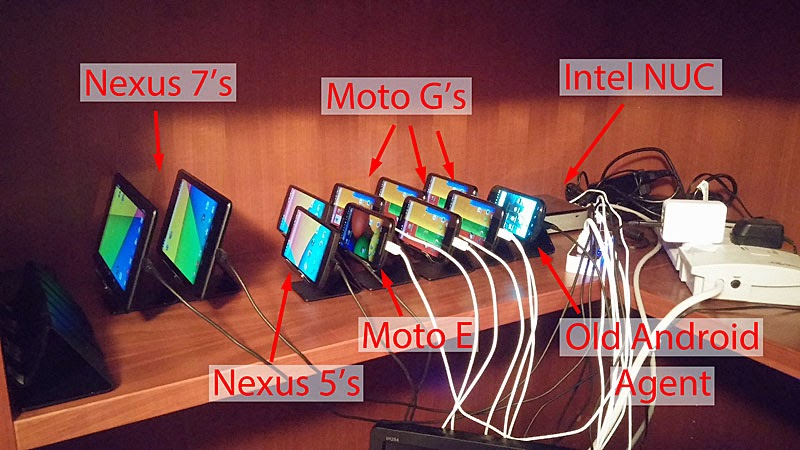
\includegraphics[width=0.5\textwidth]{wpt-android.jpg}
						\caption{Webpagtest Android device farm (Abbildung von \autocite{meenan15})}
						\label{fig:wpt-android}
					\end{center}
				\end{figure}
				\item Webpagetest hat die wohl genauste Erfassung von Netzwerkzeiten und spiegelt damit realitätsgetreu die Ladezeiten einer Seite wieder.

				\item Webpagtest liefer eine enormes Spektrum an Daten und Diagrammen, was ausführliche Analysen zulässt.

				\item Speed Index: Dies ist eine von diesem Tool eigene Maßeinheit zum bestimmen der \texttt{Perceived Performance} einer Seite.

				\begin{quote}
					\textit{"`'The Speed Index metric was added to WebPagetest in April, 2012 and measures how quickly the page contents are visually populated (where lower numbers are better).  It is particularly useful for comparing experiences of pages against each other (before/after optimizing, my site vs competitor, etc) and should be used in combination with the other metrics (load time, start render, etc) to better understand a site's performance."'}\autocite{wegpagetestDocs}
				\end{quote}

				\item Man kann Tests direkt miteinander vergleichen. Das ist möglich, indem diese URL eingegeben wird: \url{www.webpagetest.org/video/compare.php?tests=} und nach dem "`="' Zeichen die Test ID eingibt, beispielsweise "`150310\_8E\_GRH"'.
				Mit einem Komma getrennt wird eine 2. oder 3. ID angefügt. Die Tests werden dann in einer Vergleichsansicht dargestellt.

				\item Filmstrip Ansicht: Damit lässt sich visuell erkennen, wann welches Element gerendet wird.

				\item Video erstellung: Aus der Filmstrip Ansicht lässt sich ein Video erstellen. Das ist vor allem interessant, wenn mit der Vergleichsmethode mehrere Tests geladen sind. Der Ladevorgang der Testläufe wird dann in einem Video Parallel abgespielt. Vor allem für Präsentationen oder vorher / nachher Vergleiche ist dies nützlich.

				\item Test History: Durch eine Registrierung auf der Seite wird ein eigenes Testprofil angelegt in dem alle Test-ID's gespeichert werden.

				\item Testen von verschiedenen Standpunkten: Webpagetest ermöglicht es die eigene Seite von ganz verschiedenen Geographischen Standpunkten aus aufzurufen. Dadurch lässt sich ein Eindruck gewinnen, wie schnell die Seite aus dem Ausland aufrufbar ist und wie stark die Abweichung sein kann.

				\item API: Webpagtest hat eine offene API (Schnittstelle) durch die das Tool von außerhalb erreichbar ist. So lässt sich ein Test beispielsweise in Google-Spreadsheets aufrufen und das Ergebnis direkt in eine Tabelle schreiben. Mehr dazu in Punkt: \ref{..} ?. Diese Schnittstelle Limitiert allerdings die Anzahl an Tests pro Tag auf 200. Für mehr muss man sich eine eigene Private Instanz erstellen. 
				%todo ref

				\item Private Instanz: Da webpagetest Open Source ist, gibt es die möglichkeit eine eigene Private Instanz aufzusetzen. Dies kann sowohl per Amazon Cloud oder auf einem eigenen Server geschehen. Damit lassen sich dann soviele Tests ausführen, wie die Leistungs des Servers bietet.

			\end{itemize}
		% subsubsection webpagetest (end)	

		\subsubsection{Pingdom} % (fold)
		\label{ssub:pingdom}
			\url{http://tools.pingdom.com/fpt/} ist eine Alternative zu Webpagetest. Auch damit lässt sich eine URL nach Performanceproblemen analyisieren. Die Ergebnisse sind nicht so genau wie mit Webpagetest und auch ein Testen mit Smartphones fehlt. Bei einer kostenlosen Anmeldung erhält man allerdings ein System zur Überwachung der eigenen Webanwendung. Bei Ausfall oder zu hoher Last kann eine SMS versendet werden um den Admin auf diesen Umstand hinzuweisen. Durch einbetten eines Scripts auf der eigenen Seite lässt sich die Response zeit aufzeichnen (siehe Abbildung \ref{fig:choose_a_good_host}). Dieses tracking nennt man auch "`real user monitoring"' und ist zum Beispiel auch durch Google Analytics in solch einer Form abrufbar.

		
		% subsubsection pingdom (end)

		\subsubsection{Speedcurve} % (fold)
		\label{ssub:speedcurve}
			Ist ein kommerzielles Tool basierend auf Webpagetest. Es liefert einen "`life monitoring"' Service mit dem sich Webanwendungen vergleichen lassen. So kann man zum Beispiel die eigene Webanwendung dauerhaft und über einen längeren Zeitraum mit denen der Konkurenz vergleichen. 

			\begin{figure}[htbp]
				\begin{center}
					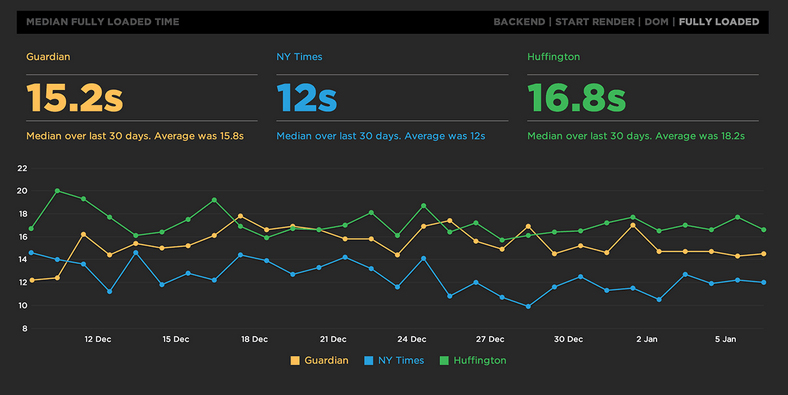
\includegraphics[width=0.7\textwidth]{speedcurve.jpg}
					\caption{Speedcurve Life Monitoring (Abbildung von \url{http://speedcurve.com/})}
					\label{fig:speedcurve}
				\end{center}
			\end{figure}

		% subsubsection speedcurve (end)

		\subsubsection{Google Spreadsheet} % (fold)
		\label{ssub:google_spreadsheet}
			Ist im Grunde wie Microsofts Excel. In Tabellen können Werte eingetragen und Berechnungen ausgeführt werden.
			Der große Vorteil an Google Spreadhseet besteht in der Möglichkeit, dass es einen Skript Editor gibt, mit dem sich kleine Programme schreiben lassen. So sind zum Beispiel API Abfragen möglich, dessen Ergebnis dann direkt in die Tabelle geschrieben werden kann.		
		% subsubsection google_spreadsheet (end)

		\subsubsection{Feed the Bot} % (fold)
		\label{ssub:feed_the_bot}
			\url{http://www.feedthebot.com/pagespeed/} bietet umfassende Artikel zu SEO und web performance. Wenn man sich mit dem Thema web performance beschäftigen möchte, ist dies eine erstklassige Anlaufstelle.
		% subsubsection feed_the_bot (end)


		\subsubsection{What Does My Site Cost?} % (fold)
		\label{ssub:what_does_my_site_cost}
			"`Was kostet es eigentlich meinene Seitenbesucher, wenn sein Datenvolumen für diesen Monat aufgebraucht ist und er pro verbrauchtes MB zur Kasse gebeten wird?"' Diese Frage versucht diese Webanwendung zu klären und visuell darzustellen.\\
			\url{http://whatdoesmysitecost.com/} benutzt die webpagetest Schnittstelle um eine eingegebene URL zu Analyisieren und berechnet aus den billigsten Anbieteren pro Land einen Preis für den Aufruf der Seite mittels Smartphone:

			\begin{quote}
				\textit{"`Prices were collected from the operator with the largest marketshare in the country and the for the least expensive plan with a (minimum) data allowance of 500 MB over (a minimum of) 30 days. Prices include taxes. Because these numbers are based on the least expensive plan, they are \textbf{best case} scenarios."'}\autocite{siteCosts}
			\end{quote}

		\begin{figure}[htbp]
			\begin{center}
				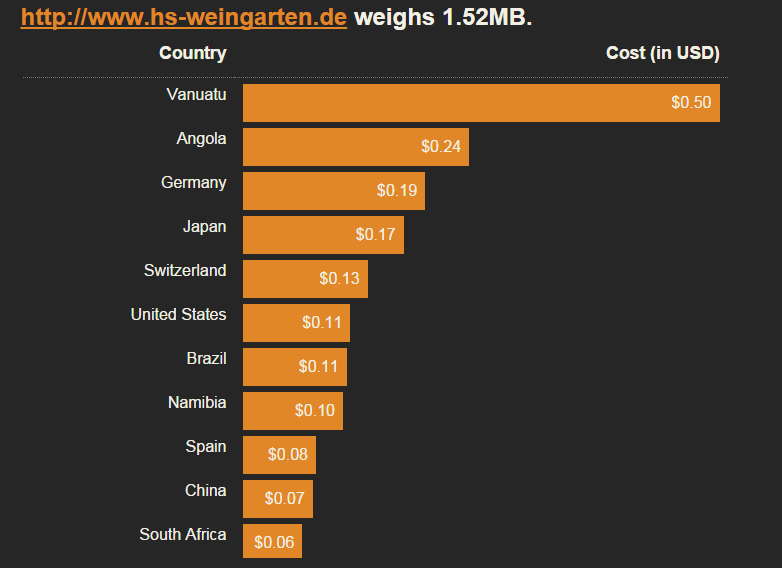
\includegraphics[width=0.7\textwidth]{what_does_my_site_cost.jpg}
				\caption{Find out how much it costs for someone to use your site on mobile networks around the world.\autocite{siteCosts}}
				\label{fig:what_does_my_site_cost}
			\end{center}
		\end{figure}

		In Deutschland kostet also der Seitenaufruf von hs-weingarten.de rund 20 Cent. Dieses Tool stellt auf sehr schöne Art und Weise dar, dass schlechte web performance nicht nur den Anwender verägert, sondern zusätzlich zum Ärger auch noch bares Geld kosten kann.
		% subsubsection what_does_my_site_cost (end)

		\subsubsection{Critical Path CSS Generator} % (fold)
		\label{ssub:critical_path_css_generator}
			Im Kapitel "`Brechen der 1000 ms Barriere"'\ref{sec:die_1000_ms_barriere} wurde gesagt, man solle das CSS des above the folds direkt in das HTML als \texttt{inline CSS} schreiben. \url{http://jonassebastianohlsson.com/criticalpathcssgenerator/} erstellt aus einer gegebener URL und dem dazugehörigen CSS genau den CSS-Code, der für den above the fold Bereich nötig ist. Das Ergebnis lässt sich dann bequem in das eigene HTML einfügen.\\

			Dieser Generator funktioniert allerdings nur dann gut, wenn sowohl die Smartphone, als auch Desktop Darstellung identisches CSS haben. Bootstrap zum Beispiel manipuliert die Navigation auf der Smartphone Ansicht per Javascript und fügt dabei Elemente ein. Diese Elemente kennt dieser Generator natürlich nicht und kann sie folglich auch nicht beachten. Eine alternative Methode wird in Kapitel ... \ref{..} ? vorgestellt.

		% subsubsection critical_path_css_generator (end)

		\subsubsection{Mozilla JPEG (alias moz jpeg)} % (fold)
		\label{ssub:moz_jpeg}
			Ist ein von Mozilla entwickelter JPEG Bild Encoder um die Bildgröße, nicht aber die Bildqualität zu verringern.

			\begin{quote}
				\textit{"`For the short term Mozilla has developed MozJPEG — a modernized JPEG encoder that offers better compression while remaining fully standard-compliant, so it’s compatible with all browsers, operating systems and native apps, and you can use it today without waiting for the whole world to upgrade"'\autocite{mozJPEG}}
			\end{quote}

			Allerdings ist die Verwendung nicht ganz so einfach wie in diesem Zitat dargestellt und es ist das eigenständige Compilieren von \texttt{C}-Code\footnote{Das Repository ist hier zu finden: \url{https://github.com/mozilla/mozjpeg} und eine Anleitung gibt es hier: \url{http://calendar.perfplanet.com/2014/mozjpeg-3-0/}} nötig, um dies auf dem eigenen Betriebssystem zu verwenden.\\
			Glücklicherweise es gibt eine Webanwendung\footnote{Webanwendung zur Verwendung von moz jpeg: \url{https://imageoptim.com/mozjpeg}} mit der ganz einfach per "`drag and drop"' Bilder mittels diesem Encoder komprimiert werden können. Je nach Bild lassen sich so mehrere Hundert Kilobyte einsparen (abhängig von der Qualitätseinstellung und größe des Bildes).
		
		% subsubsection moz_jpeg (end)

		\subsubsection{Http Archive} % (fold)
		\label{ssub:http_archive_bigqueri_es}
			\url{http://httparchive.org/} ist ein Archiv der populärsten Seiten des Internets und bietet eine Vielzahl an statistischen Auswertungen, Trends und Daten.
			\begin{quote}
				\textit{"`[HTTP Archive] is a permanent repository of web performance information such as size of pages, failed requests, and technologies utilized. This performance information allows us to see trends in how the Web is built and provides a common data set from which to conduct web performance research."' \autocite{httpArchive}}
			\end{quote}
			
		% subsubsection http_archive_bigqueri_es (end)

		\subsubsection{Perf Tooling Today} % (fold)
		\label{ssub:perf_tooling_today}
			\url{http://perf-tooling.today/} ist wohl die Umfassendste Sammlung an web performance Tools und Material im Internet. Es hat eine Liste von 105 Tools, 51 Artikel, 27 Videos und 14 Slidedecks (Stand: 12.03.15).
		
		% subsubsection perf_tooling_today (end)

		\subsubsection{Twitter} % (fold)
		\label{ssub:twitter}
			Twitter bietet die Möglichkeit am Puls der Zeit zu sein und unter dem Hashtag \#webperf und \#perfmatters erhält man neuste Erkentnisse, Tools oder Links, die sonst unentdeckt bleiben.
		
		% subsubsection twitter (end)
	\pagebreak
	% subsection tools (end)


	\subsection{Ausgangspunkt}
	\label{sub:ausgangspunkt}
		Im folgenden Abschnitt soll beschrieben werden, wie der Prozess ausgesehen hat, um von einer langsamen Webanwendung zu einer schnellen zu gelangen. Von beginn an war es wichtig, den Verbesserungsablauf zu Dokumentieren und in konkrete Daten zu fassen. Wie bereits unter Punkt \ref{ssub:google_spreadsheet} beschrieben, bietet Google Spreadsheets die möglichkeit Skripte zu schreiben und die Ergebnisse direkt in eine Tabelle auszugeben. Diesen Umstand hat sich \texttt{Andy Davies} zu nutzen gemacht und ein Programm\footnote{WebPageTest Bulk Tester via GitHub: \url{https://github.com/andydavies/WPT-Bulk-Tester}} geschrieben (MIT License), dass es ermöglicht Webpagtestest innerhalb einer Google Tabelle\footnote{Das Google Dokument ist hier zu finden: \url{http://tinyurl.com/nv4pge5}} aufzurufen. Damit wurde während der Entwicklungsphase täglich tests aufgezeichnet.\footnote{Die gesamten Daten sind hier zu finden: \url{http://tinyurl.com/l5usz79}} Die Auswertung dieser Daten erfolgt in Punkt \ref{..} ?\\
		%todo ref

		Da nur in Dulles VA eine Testinstanz mit richtigen Smartphones zur Verfügung steht, wurde mittels der \texttt{Microsoft Azure Cloud} die selbe Seite auch in den USA gehostet, um die Latenz zwischen USA und Europa zu eliminieren. Dadurch lässt sich exakter bestimmen, wie schnell ein Smartphone mit 3G Netz die Seite aufrufen kann. Leider steht keine Testinstanz mit 4G Netz zur Verfügung.\\

		Als Ausgangspunkt dient die Seite \url{http://andreaslorer.de/old/}. Zu beginn des Optimierungsprozesses gab es folgenden Ausgangspunkt (Daten via Developer Tool \& webpagetest):\\

		Desktop: \footnote{Webpagtest: \url{http://www.webpagetest.org/result/150312_Z1_18QD/}}
		\begin{itemize}
			\item 42 requests: 30 Images, 5 JS, 3 CSS, 4 other
			\item 1000 kb Seitengröße
			\item Speed Index: \textbf{3584}
			\item Start Render: \textbf{1399}  ms
			\item Load Time: 1926 ms
			\item TTFB: 690 ms
		\end{itemize}

		Mobile: \footnote{Webpagtest: \url{http://www.webpagetest.org/result/150308_A1_2W4/}}
		\begin{itemize}
			\item 17 requests: 4 Images, 5 JS, 3 CSS, 4 other
			\item 363 kb Seitengröße
			\item Speed Index: \textbf{10642}
			\item Start Render \textbf{6968} ms
			\item Load Time: 5587 ms
			\item TTFB: 1292 ms
		\end{itemize}

		Diese Werte sind nicht gut und für dieses Projekt wurden eine Start Render Zeit von weniger als eine Sekunde und ein Speed Index von unter 1000 für sowohl Mobile als auch Desktop Geräte angestrebt.\\
		Basierend auf der Anzahl an Requests, lässt sich bereits sagen, dass auch hier noch weniger einzelne Javascript und CSS Dateien möglich sind.\\

		Der erste Schritt war es, die Seitengröße zu verringert werden. Aus diesem Grund wurde das Framework gewechselt und die Seite neu Aufgebaut. Bootstrap ist zwar ein sehr populäres Framework, hat aber gerade für kleine Seiten sehr viele Komponenten, die keine Verwendung finden (oft auch als Overhead bezeichnet). Bootstrap lässt sich zwar per "`Customize"' Funktion so zusammenstellen, dass nur die Komponenten zur Verfügung gestellt werden, die für das eigene Projekt von Nöten sind, es ist aber dennoch ein Framework mit relativ großem Volumen (~30 bis 90 kb). Die Alternativen zu Bootstrap sind vielzählig. Die Entscheidung für dieses Projekt fiel auf \url{http://purecss.io/}. Dieses Framework von Yahoo ist Komprimiert gerade einmal \textbf{4 kb} groß, vollkommen responsive und kommt mit den wichtigsten Komponenten wie einer Navigations Bar, Buttons, Tabellen, Menüs und Form Elementen. Zudem benötigt es ja nach zusammenstellung der Komponenten, kein Javascript und kein JQuery. Dadurch lassen sich weiter Kilobytes als auch Requests einsparen.\\
		Da Bootstrap seine eigene Icon-Font liefert, musste hier eine Alternative gefunden werden. "`Font Awesome"'\footnote{Font-Awesome: \url{http://fortawesome.github.io/Font-Awesome/}} bietet dabei eine der umfangreichsten Icon Sammlungen im Web an und ist unter der \texttt{Open Font License} komplett frei benutzbar (auch kommerziell). Font Awesome ist mit seinen 519 Icons allerdings nicht gerade ein Leichtgewicht und kann bis zu 100 kb groß sein. Da auf der Seite \url{http://andreaslorer.de} weniger als 20 Icons zum Einsatz kommen ist der Überschuss an Bytes die keine Verwendung haben folglich enorm. Deshalb gibt es eine Webanwendung namens \url{http://fontello.com}. Damit lassen sich aus einer Vielzahl an Icons genau die wählen, die für die eigene Seite benötigt werden. Auch die Wahl aus verschiedenen Icon-Sammlungen ist möglich. Heruntergeladen wird anschließend eine ZIP-Datei. Dies folgte dazu, dass die neue Version der Seite nur noch rund 5.3 kb (plus 0.3 kb CSS) für die Icons-Fonts benötigt.\\

		Als nächstes wird die Webanwendung mittels \texttt{Pagespeed Insight}\ref{ssub:google_pagespeed_insight} Analyisert. Das Ergebnis liefert dann Anhaltspunkte, was alles zu tun ist um eine schnellere Ladezeit zu bekommen.Im folgenden soll erläutert werden, was es alles an Verbesserungen zu tun gibt und wie dies in der Praxis umgesetzt werden kann.

		% best practices anwenden
		% server konfigurieren

		% zusammenfügen mit best practices?

		\subsubsection{Render Blocking Javascript} % (fold)
		\label{ssub:render_blocking_javascript}
			Bereits unter Punkt \ref{ssub:rendering_pfad} ist das Blockierende Verhalten von Javascript und CSS angesprochen worden. Grundvoraussetzung für diesen Punkt ist, dass das Javascript der Webanwendung in ihre, für das Rendern kritische und für das Rendern unkritische Teile zerlegt wurde. 

			Der Browser stellt bereits von Haus aus zwei Attribute bereit, mit denen sich Skripte asynchron herunterladen lassen. Diese Attribute heißen "`async"' und "`defer"' und werden von jedem Browsertyp unterstützt.\autocite{canIuse} Sie erlauben es, dass der Browser nicht auf das Herunterladen der Dateien warten muss, sondern mit dem Parsen des Dokuments fortfahren darf. Async wird direkt nach dem herunterladen ausgeführt und dafür muss das Parsen pausiert werden. Defer hingegen unterscheidet sich von async in zwei Punkten: 1. Das Skripte wird nach Ende des Parsens ausgeführt. 2. Mit defer verzögert geladene Skripte werden in genau der Reihenfolge ausgeführt, wie die Reihenfolge der Skripte im HTML Dokuments vorliegen.
			
			\begin{figure}[htbp]
				\begin{center}
					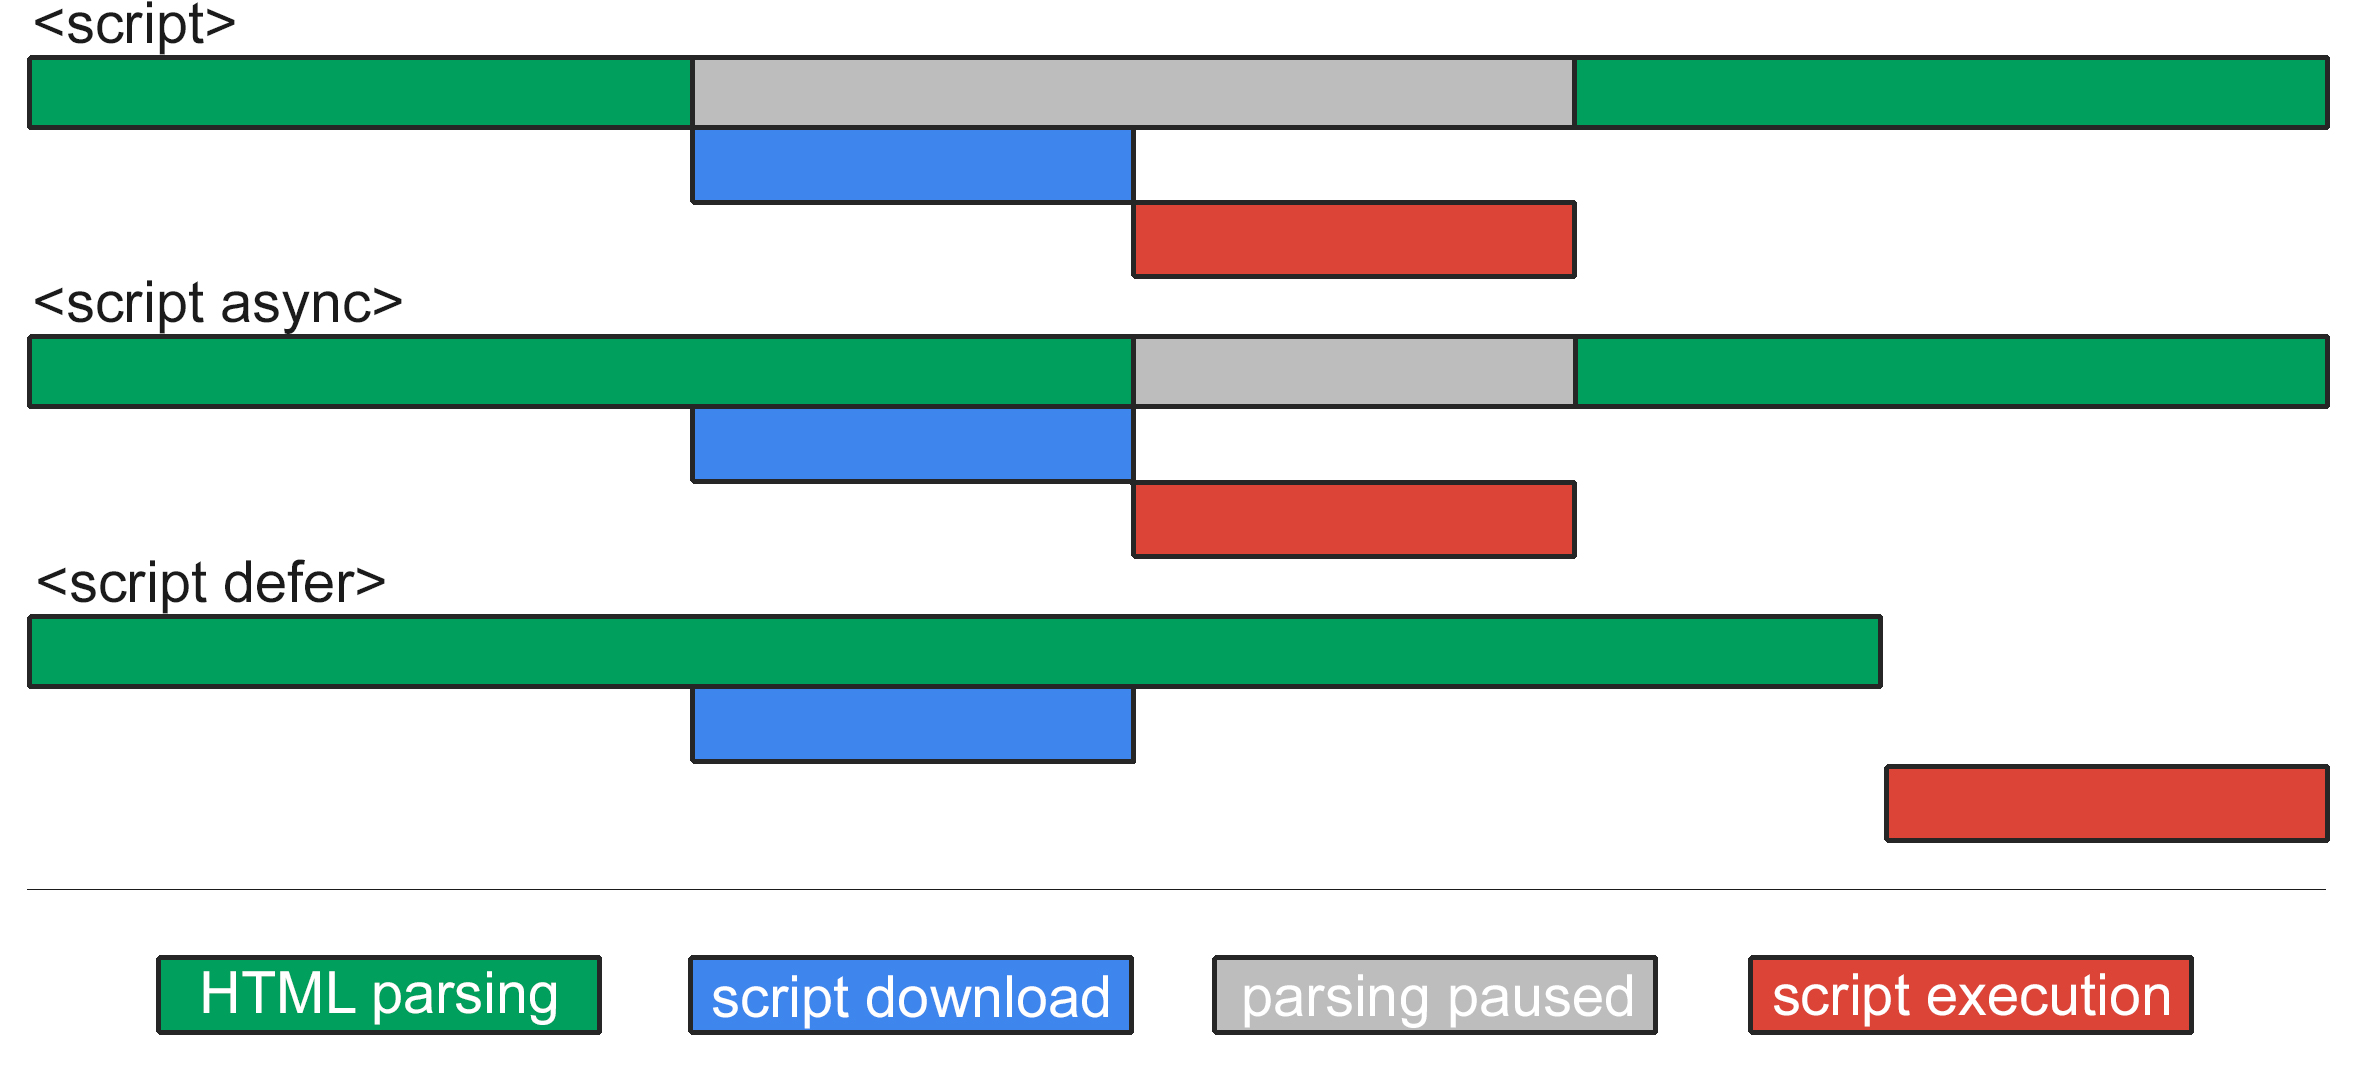
\includegraphics[width=\textwidth]{defer_scripts.jpg}
					\caption{Script-Tags mit verschiedenen Attributen (Abbildung nach \autocite{growing})}
					\label{fig:defer_scripts}
				\end{center}
			\end{figure}

			Diese Methode erlaubt es, Skripte parallel herunterzuladen, ohne dass der Renderprozess warten muss. Was damit nicht erreicht werden kann ist, dass der Download so lange verzögert wird, bis die für die Seiten primär wichtigen Ressourcen zuerst heruntergeladen wurden.\\

			Mit Hilfe des Javascripts in Listing \ref{lst:deferJs}, kann die Datei "`defer.js"' komplett mit dem Laden verzögert werden, bis der Ladeprozess der Seite abgeschlossen ist.\\
	
			\begin{lstlisting}[captionpos=b, caption=Javascript nach \autocite{deferJS}, label=lst:deferJs]
			// the function to asynchronous load js
			function loadJS( src, cb ){
				"use strict";
				var ref = window.document.getElementsByTagName( "script" )[ 0 ];
				var script = window.document.createElement( "script" );
				script.src = src;
				script.async = true;
				ref.parentNode.insertBefore( script, ref );
				if (cb && typeof(cb) === "function") {
					script.onload = cb;
				}
				return script;
			}

			// the function call to load your script
			loadJS( "path/to/script.js" );
			\end{lstlisting}

			Dieses Skript hat einen Nachteil: Es kann nicht mehrere Skripte laden, die voneinander Abhängen und deren Reihenfolge wichtig ist, um die Funktionalität zu gewährleisten. 

			\begin{quote}
				\textit{"`loadJS does nothing to manage execution order of requested scripts, so we do not advise using it to load multiple javascript files that depend on one another. It simply fetches a script and executes it as soon as possible. You can certainly use loadJS to load multiple scripts as long as those scripts are designed to execute independently of any other scripts being loaded by loadJS."'\autocite{deferJS}}
			\end{quote}

			So gibt es Skripte (Skript A) die von anderen Frameworks wie zum Beispiel JQuery (Skript B) abhängen. Das Bedeutet, wenn Skript A schneller heruntergeladen und ausgeführt wird als Skript B, Skript A bereits Funktionen von Skript B aufruft, die noch nicht zur Verfügung stehen. Daraus resultiert, dass das Skript fehlschlägt und somit teile der Webanwendung nicht mehr Funktionieren.\\

			Deshalb gibt es Skripte die genau diese Funktionalität bereistellen können. Skript A und B werden gleichzeitig heruntergeladen, Skript A wird aber erst genau dann Ausgeführt, wenn Skript B zu Verfügung steht.\\

			\url{http://headjs.com/} kann das erreichen. Durch herunterladen und einfügen in das HTML Dokument, kann per Funktionsaufruf die Abhängigkeit festgelegt werden:

			\begin{lstlisting}[captionpos=b, caption=Headjs dependency loading (Listing nach http://headjs.com/), label=lst:headjs]
				// Load up some script A and then script B
				head.load("jQuery.js", function() {
				    // Call a function when done
				    console.log("Done loading jQuery");
				    head.load('defer.js')
				});
			\end{lstlisting}

			Headjs hat den Nachteil, dass es auch noch andere Funktionalitäten außer dem Laden von Javascript ermöglicht. Dies wird aber nicht benötigt und deshalb ist Headjs mit 2.1 kb doch zu groß, um es \texttt{Inline} in das HTML Dokument zu schreiben. Eine bessere Alternative ist \texttt{jQl}. \footnote{jQl an asynchronous jQuery Loader: \url{http://www.yterium.net/jQl-an-asynchronous-jQuery-Loader}}
			Die Verwendung ist sehr Simpel:

			\begin{lstlisting}[captionpos=b, caption=jQl asynchronous jQuery-Loader, label=lst:jQl]
				<script type="text/javascript">
				  jQl.loadjQ('jquery.js');
				  jQl.loadjQdep('defer.js');
				</script>
			\end{lstlisting}

			Dieses Skript sagt im Grunde: Lade beide Dateien gleichzeitig herunter, beachte aber die Abhängigkeit (loadjQdep steht für: load dependency) von defer.js gegenüber jquery. Ist defer.js früher heruntergeladen als jquery, so wird gewartet und danach werden die Skripte in der richtigen Reihenfolge ausgeführt.\\

			Für die Webseite \url{http://andreaslorer.de} wurde sowohl defer, als auch das Skript \texttt{jQl} verwendet. "`<script defer src='critical.js'></script>"' wird dabei in den "`<head>"' bereich des HTML Dokments platziert, damit es möglichst früh erkannt wird und der Download bereits beginnen kann und das Skript aus Listing \ref{lst:jQl} befindet sich vor dem "`</body>"'-Tag.

		% subsubsection render_blocking_javascript (end)

		\subsubsection{Render Blocking CSS} % (fold)
		\label{ssub:render_blocking_css}
			Wie Javascript blockiert auch CSS das Rendern der Seite. In Listing \ref{deferCSS} ist ein Skript der Filament Group uzu sehen. Dieses Skript ermöglicht es CSS Verzögert zu laden. 

			\begin{lstlisting}[captionpos=b, caption=load a CSS file asynchronously, label=lst:deferCSS, breaklines=false]
			<script>
				// minified script after: 
				// https://github.com/filamentgroup/loadCSS/blob/master/loadCSS.js
				// [c]2014 @scottjehl, Filament Group, Inc.
				// Licensed MIT
	 			function loadCSS(e,a,g,h){function f(){for(var a,c=0;c<d.length;c++)d[c].href&&
	 				-1<d[c].href.indexOf(e)&&(a=!0);a?b.media=g||"all":setTimeout(f)}
	 				var b=window.document.createElement("link");a=a||
	 				window.document.getElementsByTagName("script")[0];
	 				var d=window.document.styleSheets;b.rel="stylesheet";b.href=e;b.media="only x";
	 				b.onload=h||function(){};a.parentNode.insertBefore(b,a);f();return b
	 			};

	  		loadCSS( "path/to/css" );
			</script>

			<!-- fallback if javascript is disabled in browser -->
			<noscript><link href="path/to/css"></noscript>
			\end{lstlisting}

			Mehr als dieses Skript ist nicht notwendig.
				
		% subsubsection render_blocking_css (end)

		\subsubsection{Inline von CSS} % (fold)
		\label{ssub:inline_von_css}
			Kleinere Mengen an CSS lassen sich direkt \texttt{Inline} in das HTML Dokument einfügen. Dadurch sind diese gleich mit dem ersten Request bereits im Dokument enthalten und müssen nicht erst angefordert und heruntergeladen werden.
		% subsubsection inline_von_css (end)

		\subsubsection{Ressourcen reduzieren} % (fold)
		\label{ssub:ressourcen_reduzieren}
			Durch das Reduzieren von Ressourcen werden unnötige Bytes entfernt. Kommentare, Leerzeichen oder Zeilenumbrüche sind für die Funktionalität nicht notwendig. Bei der Verkleinerung des HTML- CSS oder Javascript Codes werden diese entfern und dadurch die Dateigröße verkleinert.\\

			Wie unter Punkt \ref{ssub:google_pagespeed_insight} angesprochen, gibt es Pagespeed Insight auch als Chrome-Erweiterung. Damit ist es möglich, eine reduzierte Version des HTML Dokuments zu erzeugen. Für Javascript ist der Closure Compiler \ref{ssub:closure_compiler} das richtige Werkzeug. CSS lässt sich per \url{http://cssminifier.com/} verkleinern.
		% subsubsection ressourcen_reduzieren (end)

		\subsubsection{CSS-Bereitstellung optimieren} % (fold)
		\label{ssub:css_bereitstellung_optimieren}
			Wenn externe Ressourcen klein sind können diese direkt in das HTML Dokument \texttt{Inline} platziert werden. Dabei sollte darauf geachtet werden, dass das HTML Dokument Komprimiert nicht die 14 kb Marke überschreitet um es in dem ersten round trip liefern zu können. CSS Dateien die groß sind sollten sollten per \texttt{Link-Tag} eingebunden werden und mittels Skript Verzögert geladen werden.	Das CSS für den above the fold Bereich sollte \texttt{Inline} im "`<head>"' Bereich der Seite stehen. 
		% subsubsection css_bereitstellung_optimieren (end)

		\subsubsection{Bilder optimieren} % (fold)
		\label{ssub:bilder_optimieren}

		\begin{figure}[htbp]
			\begin{center}
				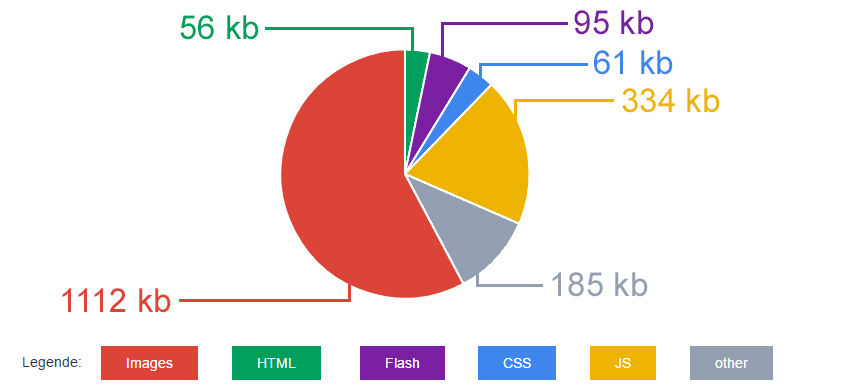
\includegraphics[width=\textwidth]{site_weight.jpg}
				\caption{Average Bytes per Page by Content Type \autocite{httpArchive}}
				\label{fig:site_weight}
			\end{center}
		\end{figure}
		
		% subsubsection bilder_optimieren (end)

		\subsubsection{Antwortzeit des Servers reduzieren} % (fold)
		\label{ssub:antwortzeit_des_servers_reduzieren}
			Die Zeit zur Antwort des Servers lässt sich zum Beispiel mit webpagteste herausfinden. Ein Server sollte auf eine Response Zeit von unter 200 ms kommen. \textit{"`Es gibt Dutzende potenzielle Faktoren, die die Antwortzeit Ihres Servers beeinträchtigen können: eine langsame Anwendungslogik, langsame Datenbankabfragen, langsames Routing, Frameworks, Bibliotheken, CPU-Ressourcenmangel oder Speicherplatzmangel. Berücksichtigen Sie zur Verkürzung der Antwortzeit Ihres Servers alle diese Faktoren."'} \autocite{google15}
		% subsubsection antwortzeit_des_servers_reduzieren (end)

		\subsubsection{Browser-Caching nutzen} % (fold)
		\label{ssub:browser_caching_nutzen}
			Fehlendes Browser-Caching (das lokale Speichern von Daten) wird von Pagspeed Insight bemängelt, wenn der Server bei seiner Antwort keinen expliziten \texttt{Caching-Header} versendet.
			Durch das Speichern von statischen Ressourcen wie Javascript, Stylesheets und Bildern kann Zeit eingespart werden, wenn der Besucher die Webanwendung ein weiteres mal aufruft. Generell sollten alle statischen Ressourchen außer das HTML Dokument selbst, gechached werden.\\

			Um auf dem Server (Apache) das Caching von statischen Ressourcen zu ermöglichen, ist ein Eintrag in die \texttt{.htaccess} Datei des Servers nötig. Folgender Eintrag sollte dort platziert werden:

		  \begin{lstlisting}[captionpos=b, caption=Aktivieren von Browser Caching in Apache (Listing nach: \autocite{sextonCaching}), label=lst:caching]
		  	## EXPIRES CACHING ##
		  	<IfModule mod_expires.c>
		  	ExpiresActive On
		  	ExpiresByType image/jpg "access 1 year"
		  	ExpiresByType image/jpeg "access 1 year"
		  	ExpiresByType image/gif "access 1 year"
		  	ExpiresByType image/png "access 1 year"
		  	ExpiresByType text/css "access 1 year"
		  	ExpiresByType text/woff "access 1 year"
		  	ExpiresByType application/pdf "access 1 year"
		  	ExpiresByType text/x-javascript "access 1 year"
		  	ExpiresByType application/x-shockwave-flash "access 1 year"
		  	ExpiresByType image/x-icon "access 1 year"
		  	ExpiresDefault "access 1 month"
		  	</IfModule>
		  	\#\# EXPIRES CACHING \#\#
		  \end{lstlisting}

		  Listing \ref{lst:caching} hat 2 Aufgaben. Erstens: Es setzt die Ablaufzeit für alle statischen Ressourcen auf 1 Jahr und erfüllt damit den von Google empfohlenen Wert. Längere Speicherzeiten sind dagegen nicht Empfohlen, da dies gegen die RFC-Richtlinien verstoßen würde \autocite{google14Caching}. Zweitens: Es wird mit dem HTTP Request ein Header mit gesendet. Dieser ermöglicht es dem Browser seine lokal gespeicherten Ressourcen zu managen. Er besteht aus folgenden Teilen und es ist jeweils nur \textbf{eine} der Optionen nötig.

		  \begin{itemize}
		  	\item Last-Modified: date
		  	\item ETag: ID
		  \end{itemize}

		  Diese beiden Header ermöglichen es dem Browser zu überprüfen, ob sich die gecachten Ressourcen geändert haben oder noch identisch sind. Last-Modified ist dabei das Datum der letzten Änderung und beim ETag-Header handelt es sich um einen automatisch generierten Wert der die Datei eindeutig Identifiziert.\\
		  Beim erneuten Laden einer Seite werden diese Header zurück an den Server gesendet und verglichen. Wenn die Datei auf dem Server geändert wurde stimmen die Werte nicht überein und der Server schickt eine entsprechende Antwort zurück.

		  \begin{itemize}
		  	\item Cache-Control: max-age=value
		  	\item Expires: date
		  \end{itemize}

		  Mit diesen Headern ist es möglich Serveranfragen komplett zu vermeiden. Das bedeutet, dass die Latenz bei Smartphones komplett negiert werden kann, indem Requests an den Server erst gar nicht stattfinden müssen. "`Sämtliche vom Browser ausgegebenen HTTP-Anfragen werden zuerst an den Browsercache weitergeleitet, um zu überprüfen, ob eine gültige Antwort im Cachespeicher vorliegt, die der Anfrage entspricht. Liegt eine Übereinstimmung vor, wird die Antwort aus dem Cache ausgelesen, wodurch sowohl die Netzwerklatenz als auch die durch die Übertragung anfallenden Datenkosten umgangen werden."'\autocite{grigorikCaching} Gültige Ressourcen werden erst gar nicht angefragt, sondern gleich aus dem Cache geladen. Ungültige oder abgelaufene Ressourcen werden dagegen vom Server geholt. Ohne diesen Header, muss der Browser für jede in seinem Cache befindliche Ressource, den Server anfragen. Dafür sind jedes mal ein round trip nötig (3G = 300ms).\\

		  \begin{figure}[htbp]
		  	\begin{center}
		  		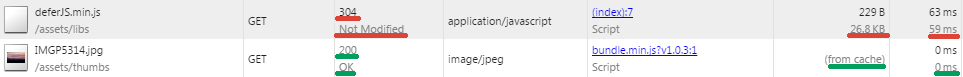
\includegraphics[width=\textwidth]{caching_enabled.jpg}
		  		\caption{Gecachte Ressourcen müssen nicht mehr abgefragt werden}
		  		\label{fig:caching_enabled}
		  	\end{center}
		  \end{figure}
		  
		  Das rot unterstrichene zeigt, dass 59 ms im Netzwerk verbraucht wurde (Kabel Verbindung). Der Server antwortete mit: "`Not-Modified"'. Grün zeigt, dass keinerlei Kommunikation mit dem Server nötig ist sondern die Datei, in diesem Fall ein Bild, direkt aus dem Cache geholt wird.\\
		 
		  Was aber wenn sich zum Beispiel eine CSS-Datei geändert hat? Dann würden nun Besucher mit leerem Cache eine andere Darstellung erhalten wie Besucher mit der gecachten Version. Dafür gibt es mehrere Lösungsansätze.

		  \begin{enumerate}
		  	\item Die HTML Datei sollte nicht gecached werden da sonst Änderungen nicht mehr den Anwender können.
		  	\item Eine für die Datei angemessene max-age: Dateien die sich oft ändern dürfen auch entsprechend niedrige max-age Werte haben. Dadurch wird die Datei Zeitnah für alle Anwender neu Angefordert.
		  	\item Ressourcen können mit einer ID versehen werden: \texttt{styles.css} wird in \texttt{styles.v1.0.1.css} umbenannt.
		  	\item Alternativ zur ID ist auch in \texttt{Fingerprint} möglich. Dabei wird eine ID aus der Datei generiert. Ändert sich die Datei so ändert sich auch der Fingerprint. Dieser Fingerprint wird auch wiederrum dem Dateiname angefügt. Das kann so aussehen: \texttt{styles.82s0dfsa.css}.\footnote{Dieses Verfahren lässt sich auch automatisieren, ich verweise auf folgenden Artikel: \url{https://adactio.com/journal/8504}}
		  \end{enumerate}

		  Browser-Caching ist eine mächtige Funktionalität die sich jeder zu nutzen machen sollte. Sie ist zudem ganz einfach mit nur einem Eintrag in die \texttt{.htaccess}-Datei realisierbar. Allerdings hat eine Studie von Yahoo ergeben, dass 40-60\% der Besucher beim Seitenaufruf einen leeren Cache haben und rund 20\% aller aufgerufenen Seiten wurden mit einem leeren Cache aufgerufen.
			\begin{quote}
				\textit{"`[...] I don't know about you, but these results came to us as a big surprise. It says that even if your assets are optimized for maximum caching, there are a significant number of users that will always have an empty cache."'\autocite{yahoo07}}
			\end{quote}

			Folglich macht es Sinn, die Geschwindigkeit der Seite für die sogenannten "`first users"' zu optimieren und nicht von einer gecachten Version der Seite auszugehen.\\
			Mittels dem Tool: \url{http://www.feedthebot.com/tools/if-modified/} lässt sich überprüfen, ob die eigene Webseite "`Browser-Caching"' richtig einsetzt. 
		  \begin{figure}[htbp]
		  	\begin{center}
		  		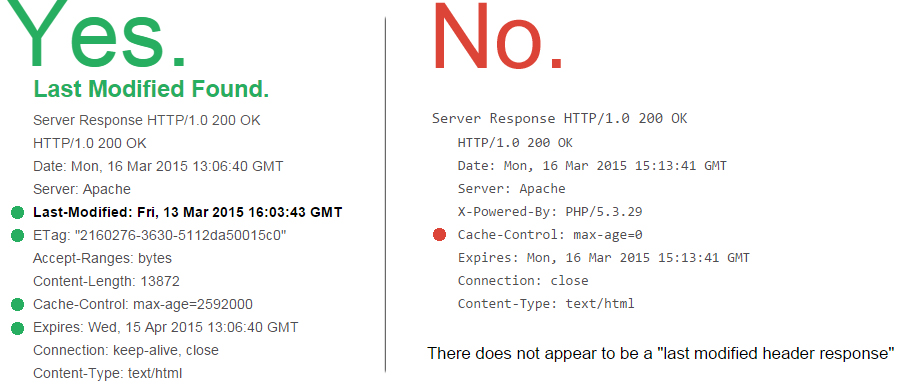
\includegraphics[width=\textwidth]{expires_header.jpg}
		  		\caption{Beispiel: Eine Webseite mit und ohne "`Cache Control"'. (Eigene Abbildung nach \url{http://www.feedthebot.com/tools/if-modified/})}
		  		\label{fig:expires_header}
		  	\end{center}
		  \end{figure}
		% subsubsection browser_caching_nutzen (end)

		\subsubsection{Komprimierung aktivieren} % (fold)
		\label{ssub:komprimierung_aktivieren}
		\begin{lstlisting}[captionpos=b, caption=gzip, label=lst:gzip]
			## gzip Compression if availiable
			<ifModule mod_gzip.c>
			mod_gzip_on Yes
			mod_gzip_dechunk Yes
			mod_gzip_item_include file \.(html?|txt|css|js|php|pl)$
			mod_gzip_item_include handler ^cgi-script$
			mod_gzip_item_include mime ^text/.*
			mod_gzip_item_include mime ^application/x-javascript.*
			mod_gzip_item_exclude mime ^image/.*
			mod_gzip_item_exclude rspheader ^Content-Encoding:.*gzip.*
			</ifModule>
		\end{lstlisting}
			
		% subsubsection komprimierung_aktivieren (end)

		\subsubsection{Keep Alive ermöglichen} % (fold)
		\label{ssub:keep_alive_ermöglichen}
		\begin{lstlisting}[captionpos=b, caption=keep alive, label=lst:keepAlive]
			# keep-alive
			<ifModule mod_headers.c> 
			Header set Connection keep-alive
			</ifModule>
		\end{lstlisting}
			
		% subsubsection keep_alive_ermöglichen (end)

	% subsection ausgangspunkt (end)

	\subsection{Prozess der Validierung}
	\label{sub:prozess_der_validierung}
	
	% subsection prozess_der_validierung (end)

	

% section entwicklung (end)